\section{Business Model}

\begin{figure}[H]
  \centering
  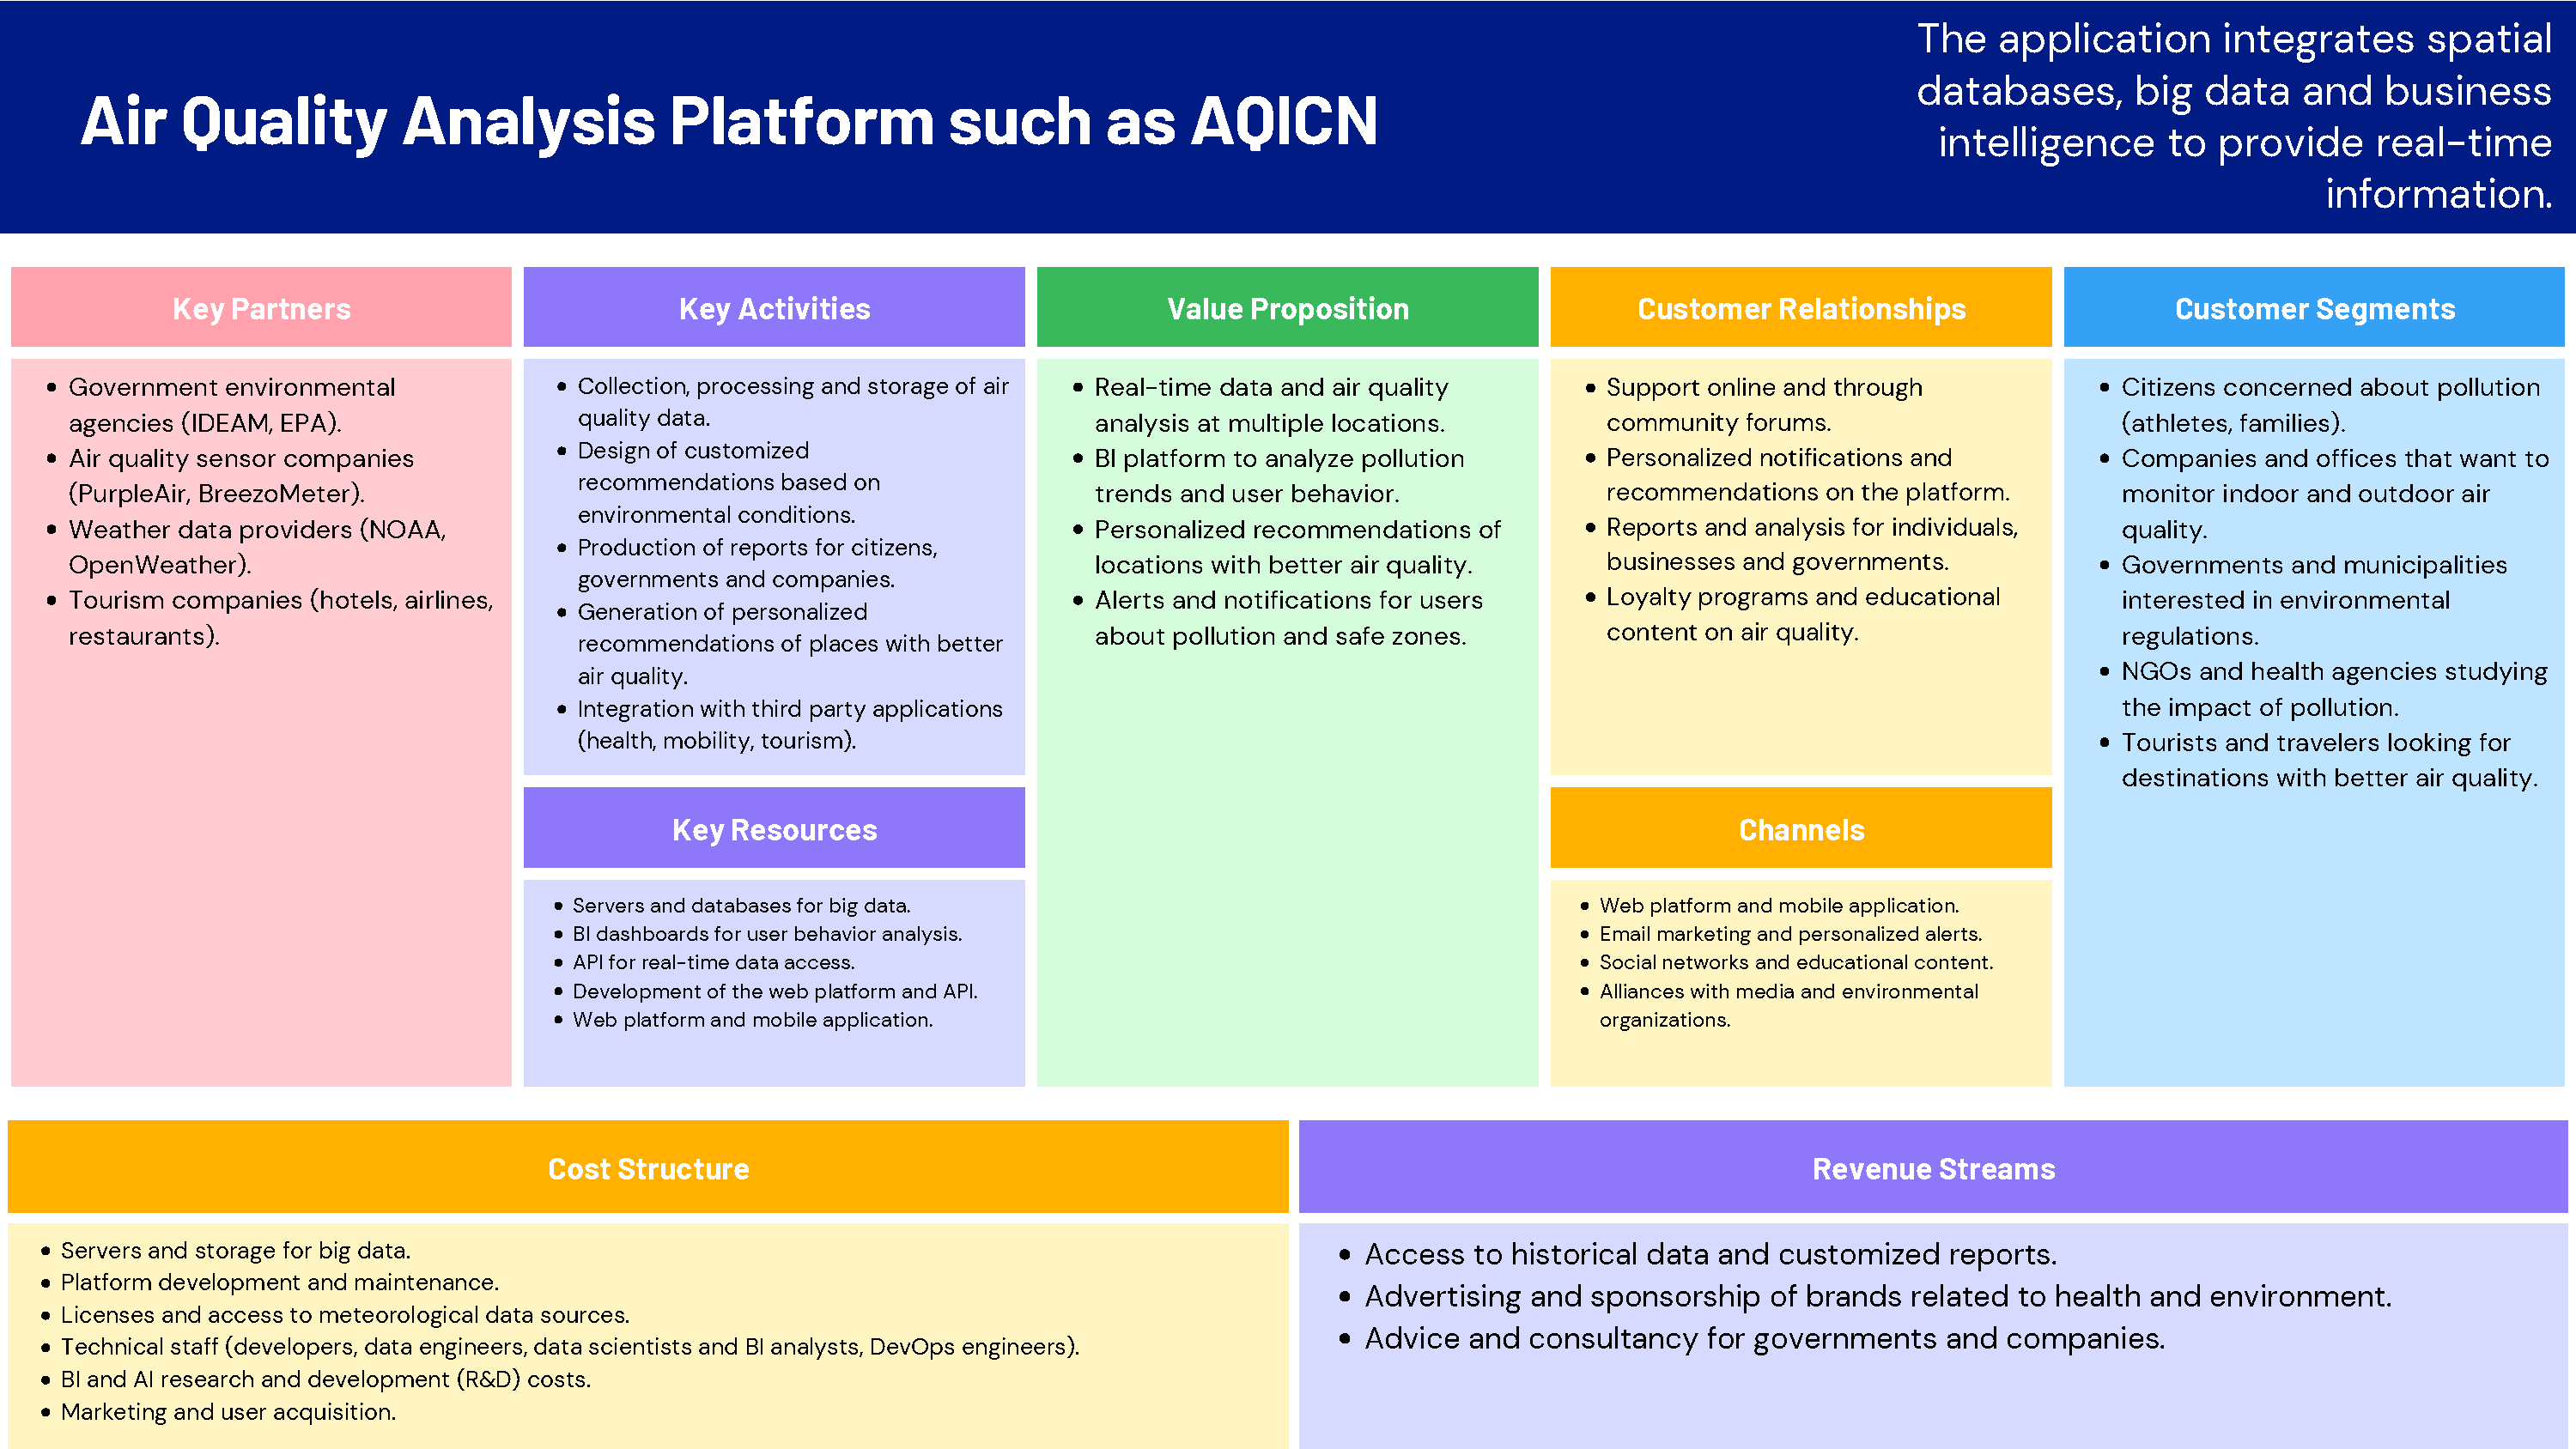
\includegraphics[width=\linewidth]{Imagenes/Business_Model.pdf}
  \caption{Business Model}
\end{figure}

\subsection*{How Does It Work?}
The platform operates through the following process:

\begin{itemize}
  \item It collects data from environmental sensors and third-party APIs (such as meteorological stations and air quality sensors).
  \item It processes the data to clean, transform, and store it in both relational and big data databases.
  \item It displays useful information to users through:
    \begin{itemize}
      \item Real-time dashboards.
      \item Personalized recommendations.
      \item Downloadable reports.
      \item Interactive maps and graphs.
    \end{itemize}
\end{itemize}

\subsection*{Who Uses the Platform?}
\begin{itemize}
  \item Citizens who want to know if it is safe to exercise or go outdoors during high pollution periods.
  \item Governments that issue alerts and design public policies.
  \item Companies and NGOs interested in analyzing environmental impact.
\end{itemize}

\subsection*{How Does It Generate Revenue?}
\begin{itemize}
  \item Through advertising from brands related to health and the environment.
\end{itemize}

\subsection*{What Technologies Does It Use?}
\begin{itemize}
  \item Relational databases (SQL) and NoSQL (for real-time data).
  \item Business Intelligence (BI) modules.
  \item APIs to allow other systems to access the data.
  \item Architecture designed for high availability, scalability, and multi-region/multi-device access.
\end{itemize}
\newpage